\documentclass{beamer}
\usetheme{Madrid}
\usepackage{palatino}
\usepackage{tikz}
\usepackage{graphicx}

\usepackage[T1]{fontenc}
\usepackage[utf8]{inputenc}
\usefonttheme[onlymath]{serif}

% Définition de l'environnement pour la figure d'Awalé avec un nombre variable de paramètres pour les pierres

\date[]{}
\title[La recherche du meilleur coup.]{À la recherche du meilleur coup au jeu d'Awalé}
\author[Nils Lelorieux]{Nils Lelorieux}
\institute[]{numéro de candidat : 24296}

\begin{document}

\begin{frame}
  \titlepage
\end{frame}
 
\begin{frame}
  \frametitle{Introduction}


  \begin{minipage}[b]{0.3\linewidth}
    \begin{figure}
      \centering
      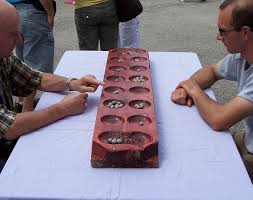
\includegraphics[width=1.5\linewidth]{ressources/photo_joueur_awale.jpeg}
      \caption{Une partie d'Awalé}
      \label{fig:mon_image}
      %% \label{fig:1}
    \end{figure}
  \end{minipage}
  \hfill
  \begin{minipage}[b]{0.48\linewidth}
    \begin{figure}
      \centering
      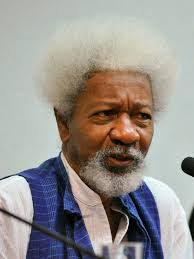
\includegraphics[width=0.8\linewidth]{ressources/wole_soyinka.jpeg}
      \label{fig1}
      \caption{Photographie de Wole Soyinka}
    \end{figure}
  \end{minipage}
      
\end{frame}

\begin{frame}
  \frametitle{Un jeu ancien et important}
  \begin{figure}
    \centering
    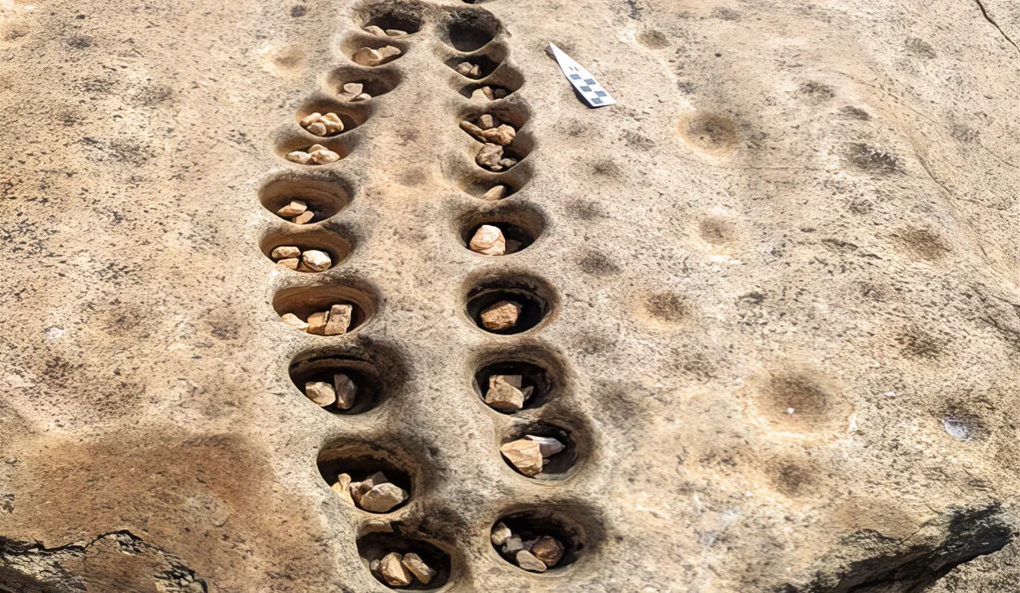
\includegraphics[width=\linewidth]{ressources/ancien_plateau_jeu.png}
    \caption{Un ancien plateau de jeu découvert au Kenya}
  \end{figure}
\end{frame}


\begin{frame}
  \frametitle{Vue d'ensemble}
  \tableofcontents
\end{frame}


\section{Présentation des règles du jeu et motivations}
\begin{frame}
  \frametitle{Règles du jeu}
  \begin{minipage}[t]{0.5\linewidth}
    \begin{itemize}
    \item<Règles du jeu>
    \item Deux joueurs s'affrontent.
    \item 4 graines dans les 12 trous divisé en 2 rangée de 6.
    \item Le premier joueur choisi un puit et sème les graines.
    \item Si le dernier puit semé a 2 ou 3 pierres, il les récupère et fait la même chose dans le puit précédent, ...
      \item Le gagnant est le joueur qui a le plus de pierres
    \end{itemize}
  \end{minipage}
  \hfill 
  \begin{minipage}[t]{0.49\linewidth}
    \begin{figure}
      \centering
      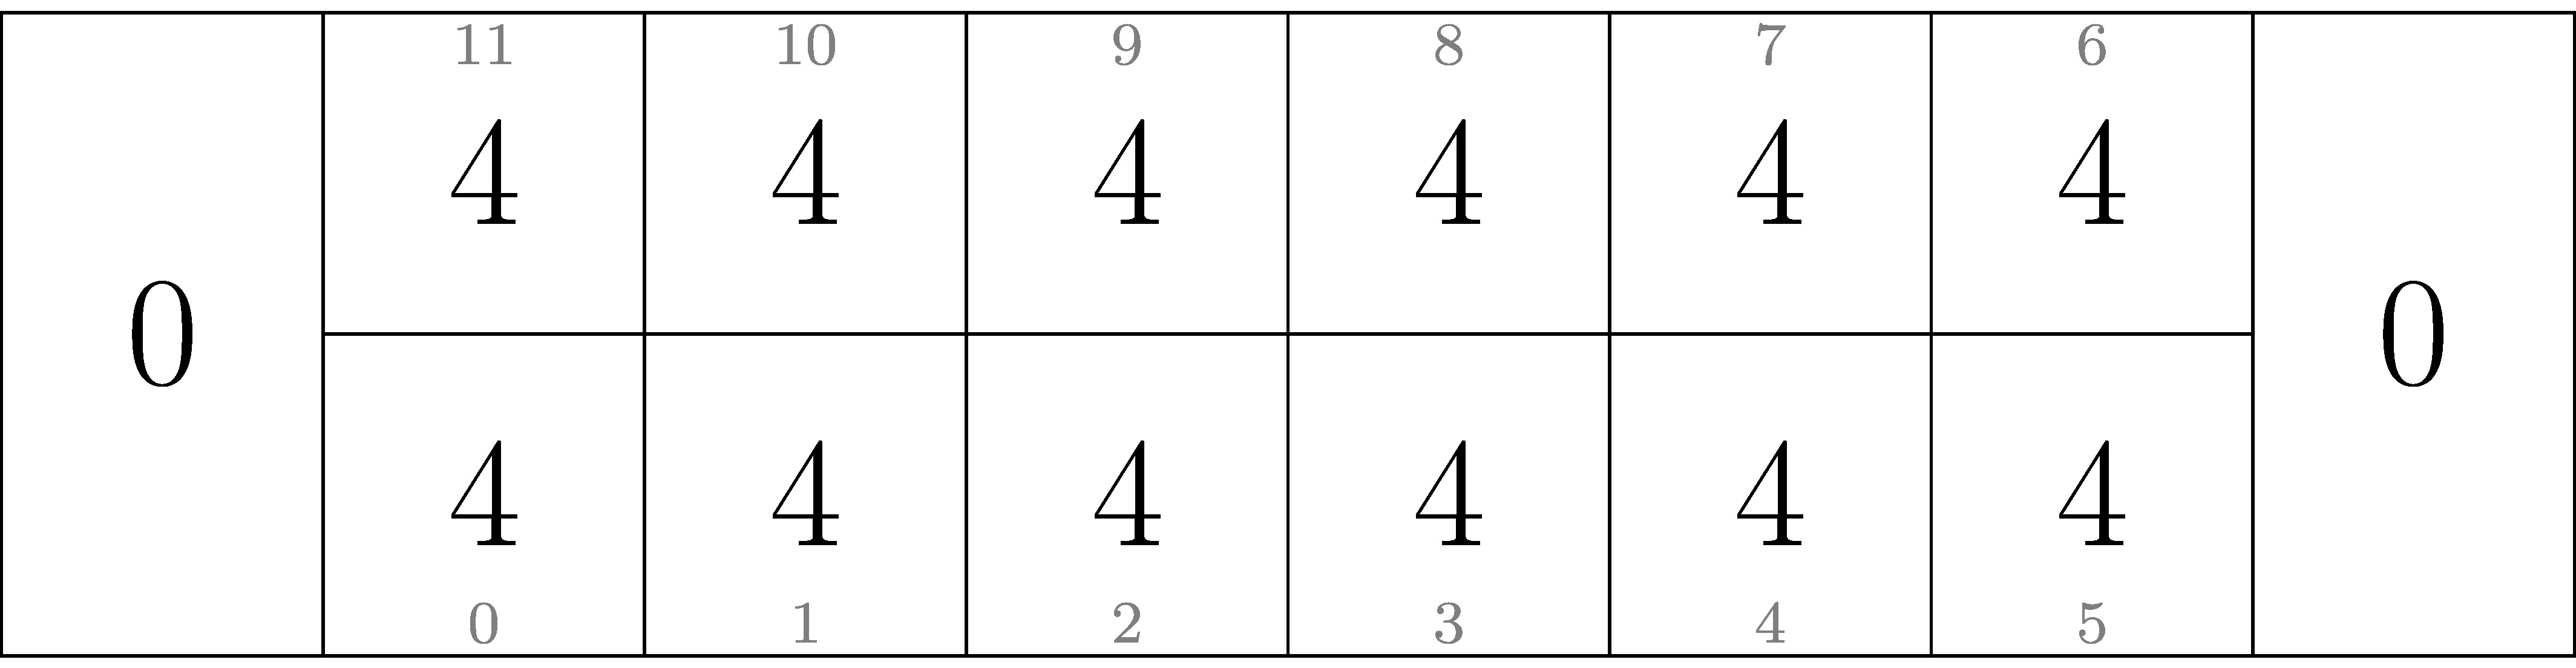
\includegraphics[width=1.05\linewidth]{ressources/p_debut.jpg}
      \caption{L'état du plateau au début de la partie}
    \end{figure}
    
  \end{minipage}
  
\end{frame}

\begin{frame}
  \frametitle{Déroulé d'une partie}
  \begin{minipage}[b]{0.45\linewidth}
    \begin{figure}
      \centering
      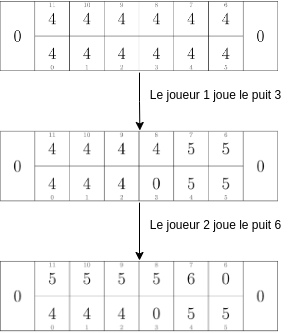
\includegraphics[width=1\linewidth]{ressources/diagramme1.png}
      \caption{2 coups joués par les 2 joueurs en début de partie}
    \end{figure}
  \end{minipage}
  \hfill
  \begin{minipage}[b]{0.45\linewidth}    
    \begin{figure}
      \centering
      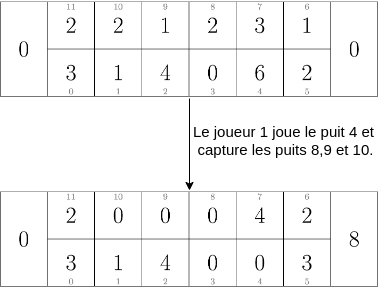
\includegraphics[width=1\linewidth]{ressources/diagramme2.png}
      \caption{Position où le joueur 1 capture les pierres du joueur 2}
    \end{figure}
  \end{minipage}
\end{frame}

\begin{frame}
  \frametitle{Motivations}
  \begin{itemize}
  \item Le facteur d'embrachement est assez faible.
  \item Possibilité d'utiliser des algorithmes classiques de la théorie des jeux pour trouver le coup optimal
  \item Il y a moins de $10^{14}$ états possibles.
  \end{itemize}
\end{frame}

\section{Échec de l'approche théorique et des premiers algorithmes}
\begin{frame}
  \frametitle{Une approche théorique}
  \begin{figure}
    \centering
    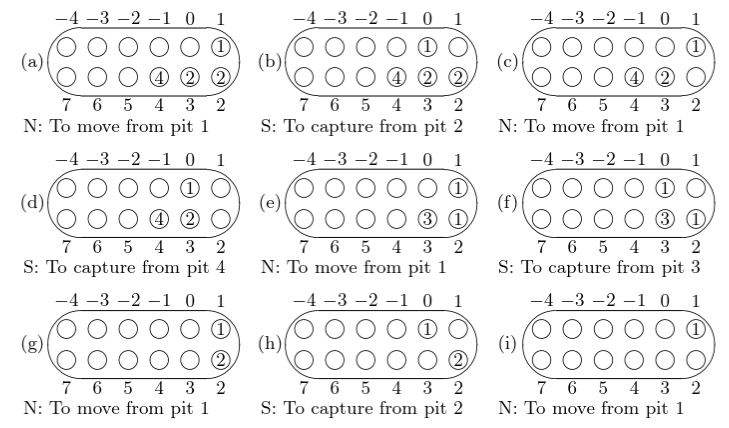
\includegraphics[width=\linewidth]{ressources/determined_positions.png}
    \caption{Un position déterminée}
  \end{figure}
\end{frame}

\begin{frame}
  \frametitle{L'algorithme min-max}
  Insérer un schéma de min max
\end{frame}


\begin{frame}
  \frametitle{Problème du min-max classique}
  \begin{figure}
    \centering
    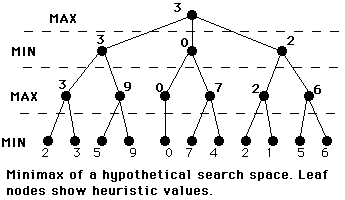
\includegraphics[width=0.8\linewidth]{ressources/min_max_heuristique.png}
    \caption{Un exemple de min max avec heuristique}
  \end{figure}
\end{frame}

\begin{frame}
  \frametitle{Résultat min-max}
  Insérer les résultats
\end{frame}

\begin{frame}
  \frametitle{Un algorithme de Monte Carlo}
  \begin{figure}
    \centering
    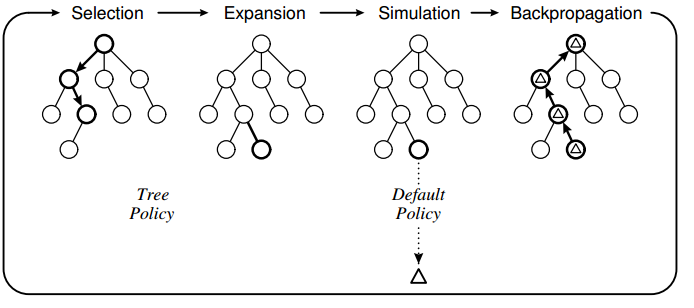
\includegraphics[width=\linewidth]{ressources/monte_carlo_explication.png}
    \caption{Principe de l'algorithme de Monte Carlo}
  \end{figure}
\end{frame}

\begin{frame}
  \frametitle{Des résultats peu convaincants}
  Insérer les résultats
\end{frame}

\section{Des résultats concluents grâce à deux nouvelles techniques : la recherche arborescente de Monte-Carlo et l'analyse rétrograde}
\begin{frame}
  \frametitle{Une amélioration de l'algorithme précédent}
  \begin{figure}
    \centering
    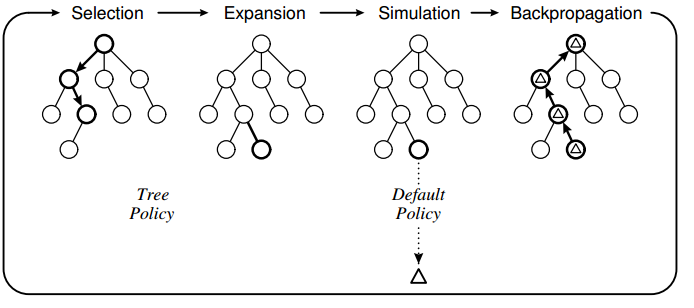
\includegraphics[width=\linewidth]{ressources/monte_carlo_explication.png}
    \caption{Principe de la recherche arborescente de Monte Carlo}
  \end{figure}
\end{frame}

\begin{frame}
  \frametitle{Comment choisir le noeud à explorer ?}
  On attribue à chaque noeud $n$ un score Q qui correspond à la moyenne des gains remportés part toutes les parties contenant le noeud $n$. Étant donné un noeud $n$ et son père $p$, on a :
  $$ Q(n) = \frac 1 {N(n)} \sum_{i=1}^{N(p)}\mathbb I_i(n)z_i $$
\end{frame}




\end{document}

%%% Local Variables:
%%% mode: LaTeX
%%% TeX-master: t
%%% End:
